\chapter{Project Context, Problem Statement, and Methodology}

\section*{Introduction}
\addcontentsline{toc}{section}{Introduction}

The present chapter establishes the foundational context within which this project was conducted. It begins by introducing the host organization, Mantu Group and its consulting subsidiary Amaris Consulting, along with the client operational environment of Orange France, specifically its Directorate of Technology, Operations, and Fixed Networks (DTOF/DINFRA). The collaboration framework between Amaris and Orange is then examined, with particular attention to the portfolio of projects delivered under this partnership and the specific unit that motivated this work, namely the Guichet OI PAR France department. The chapter subsequently provides a systematic analysis of the operational challenges faced by the OSA sub-team, identifies the structural inefficiencies of the current manual workflows, and presents the proposed solution together with its formally prioritized project objectives. It concludes with a description of the governance model, the hybrid project methodology adopted, and the planning strategy that structured the twenty-five weeks of this internship.

\section{Host Organization and Operational Environment}

This internship was conducted within Amaris Consulting, a consulting and professional services firm specializing in engineering, technology, and digital transformation. Amaris Consulting operates as an integral brand within the Mantu Group, an independent international consulting organization founded in 2007 and headquartered in Geneva, Switzerland. The Mantu Group deploys a community of more than 10,000 professionals across over 60 countries on five continents, generating annual revenues in the region of 810 million euros. The following subsections present the organizational structure of the Mantu Group, the Amaris Consulting market positioning, and the Orange France operational environment in which this project was conducted.

\subsection{The Mantu Group and Amaris Consulting}

The Mantu Group operates through a portfolio of specialized brands, each addressing a specific domain within the broader consulting and talent management ecosystem. This multi-brand architecture enables the group to serve a wide range of industries, including telecommunications, energy, banking, insurance, and public services, while preserving the organizational agility and client proximity that characterize its market identity.

\begin{figure}[H]
  \centering
  
\includegraphics[width=0.85\textwidth,max width=\textwidth]{images/image1.png}
  \caption{Organizational structure of the Mantu Group brand portfolio}
  \label{fig:image1}
\end{figure}

The principal brands comprising the Mantu portfolio at the time of this internship include the following entities. Amaris Consulting delivers engineering, technology, and digital transformation consulting services and constitutes the brand directly relevant to this project. LittleBig Connection provides a platform for managing external talent and freelance resources. Elevenvms operates as a vendor management system for contingent workforce management. Portalia is an HR and recruiting platform specializing in assessment and candidate management. Novelab is a digital innovation studio focused on design and interactive technology solutions. ARNEOD provides consulting services oriented toward organizational performance and digital transformation.

Since its founding in 2007, Amaris Consulting has undergone rapid international expansion across Europe, Asia, Africa, the Middle East, and the Americas. In 2017, the company established its first North African office in Tunisia. In the telecommunications sector, Amaris Consulting maintains a privileged partnership with Orange France, particularly in the management of fiber connection requests through the Guichet OI Infrastructure Operator Interface. Within the Mantu Group, Amaris operates a dedicated telecommunications department bringing together several hundred professionals with expertise in FTTH, FTTO, FTTA, radio engineering, project management, audit and compliance, and High Level and Low Level Design engineering.

\begin{figure}[H]
  \centering
  
\includegraphics[width=0.85\textwidth,max width=\textwidth]{images/image2.png}
  \caption{Amaris Consulting logo and international positioning within the Mantu Group}
  \label{fig:image2}
\end{figure}

\subsection{Orange France: Directorate of Technology, Operations, and Fixed Networks}

Orange is one of the world's leading telecommunications operators, present in 26 countries and serving over 310 million customers worldwide. In France, Orange is the undisputed leader in fiber optic deployment and adoption. The company was the first European operator to surpass 10 million fiber subscribers in its domestic market, with its FTTH customer base reaching approximately 15 million subscribers, significantly ahead of competitors SFR, Free, and Bouygues Telecom. Orange has deployed fiber infrastructure to over 38 million premises across France, covering approximately 80 percent of the national population, and has been ranked first in fiber network quality by ARCEP, the French telecommunications regulator, for five consecutive years.

Orange has served as the primary private-sector driver behind France's Plan France Tres Haut Debit, the national initiative targeting universal fiber coverage. This industrial-scale deployment, representing cumulative investment exceeding 15 billion euros, has positioned France among Europe's leaders in fiber network penetration. Within Orange France, the Direction Technique Operations et Fonctions (DTOF) oversees the implementation of network infrastructure projects, including fiber deployments under new real estate and renovation programs. The Direction DINFRA, operating under DTOF, is specifically responsible for managing fiber connection requests for new buildings, a process involving Infrastructure Operator consultants, internal processing agents, and business tools including Agilis, SharePoint, and Microsoft Planner.

\begin{figure}[H]
  \centering
  
\includegraphics[width=0.85\textwidth,max width=\textwidth]{images/image3.png}
  \caption{Simplified organizational chart of Orange France highlighting DTOF and DINFRA}
  \label{fig:image3}
\end{figure}

\subsection{The Amaris--Orange Consulting Engagement}

The Amaris--Orange collaboration is structured as a nearshore delivery engagement in which Amaris Consulting provides embedded consulting capacity to Orange France's fiber deployment program. Under this service contract, dedicated Amaris consultants are integrated into Orange operational units, primarily the Guichet OI PAR France unit, where they execute production tasks under a dual governance model. People management is handled by the Amaris Team Manager, while delivery management covering scope, quality, and prioritization is owned by the Service Delivery Manager, who serves as the single point of contact with Orange leadership. Weekly operational reviews between Orange and Amaris ensure alignment and continuous accountability.

To execute their operational missions, Amaris consultants are granted full access to Orange's internal platform suite spanning the fiber deployment lifecycle. This suite encompasses request and workflow management tools including Agilis, A2PO, and eTask; network production tracking systems such as Portail Production Reseau, IPON PROD G4, and Banbou-Production; geospatial referencing platforms including Georeso and Elimap; field operations coordination tools such as Backpack, Cactus, and Alcatraz; and business intelligence systems covering New Gedaffaires, Genergy, and ISCORE. This deep integration enables consultants to manage fiber connection requests, track project status in real time, and coordinate directly with Orange departments and field technicians across France.

\section{The Guichet OI Unit: PAR France Operations}

The Guichet OI PAR France unit constitutes the direct operational context of this project. This section presents the portfolio of projects managed under the Amaris--Orange partnership, then details the mission, service delivery models, organizational structure, workload profile, and manual workflows that characterize the unit.

\begin{table}[H]
  \centering
  \caption{Portfolio of projects delivered under the Amaris--Orange collaboration}
  \renewcommand{\arraystretch}{1.3}
  \begin{tabularx}{\textwidth}{|X|X|}
    \hline
    \textbf{Project} & \textbf{Description} \\ \hline
    Accueil Fibre & First point of contact for all incoming fiber-related requests from real estate operators. \\ \hline
    Plan Poteau & Pole-based infrastructure planning for aerial fiber deployment. \\ \hline
    Rami & Small-scale FTTH real estate operations for minor buildings and installations. \\ \hline
    TSO (Transfert Service Optique) & Manages fiber faults on the Infrastructure Operator network, escalating tickets and coordinating field subcontractors across Ile-de-France. \\ \hline
    B2B FTTO & Provides dedicated, unshared fiber links for enterprises, data centers, and professional environments. \\ \hline
    CRECO & Processes address creation and modification in Orange's network referential, assigning each address a unique IMB identifier required for fiber activation. \\ \hline
    Guichet OI: PAR France & Central unit within DINFRA managing real estate fiber connection requests across France. This is the focal project of this internship. \\ \hline
  \end{tabularx}
\end{table}

\subsection{Operational Mission and Service Models (OSA / OCC)}

The Guichet OI PAR France unit serves as the central entry point for all real estate fiber connection requests addressed to Orange France's DINFRA division. It coordinates the work of consultants processing incoming demands across two distinct operational models that coexist within the same team structure, each imposing different documentation, validation, and coordination requirements.

Under the Fiber OSA model, Orange assumes both the role of infrastructure operator and service provider, resulting in a vertically integrated processing chain where all decision authority resides within a single organizational entity. Under the Fiber OCC model, the infrastructure remains operated by Orange while service provision is entrusted to a third-party operator, introducing an additional coordination layer and differentiating the processing requirements for each file. The coexistence of these two models significantly increases workflow complexity and necessitates a differentiated processing approach at each stage of the connection request lifecycle.

\subsection{Organizational Structure and Workload Baseline}

The Amaris team deployed at the Guichet OI operates within a clearly defined three-level management structure that separates project delivery responsibilities from personnel management. This organizational design ensures that operational performance and individual professional development are each addressed by a dedicated point of contact within the governance hierarchy.

\begin{figure}[H]
  \centering
  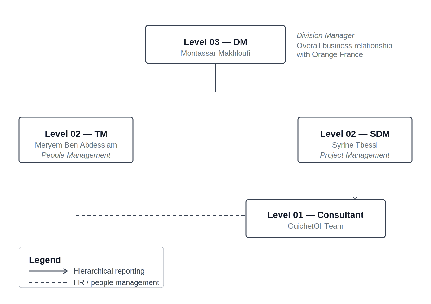
\includegraphics[width=0.85\textwidth,max width=\textwidth]{images/image4.png}
  \caption{Organizational management structure of the Amaris team at Guichet OI PAR France}
  \label{fig:image4}
\end{figure}

The full Amaris team at the Guichet OI comprises 27 consultants. The OSA processing sub-team, consisting of 15 consultants, handles the daily intake and processing of real estate fiber connection requests. The automation solution developed in this internship specifically targets this 15-person OSA sub-team, addressing the workflows that currently represent the largest share of their productive time. The remaining team members operate on OCC-related tasks and other administrative functions outside the scope of this project.

\begin{table}[H]
  \centering
  \caption{Critical operational performance indicators of the OSA sub-team}
  \renewcommand{\arraystretch}{1.3}
  \begin{tabularx}{\textwidth}{|X|X|}
    \hline
    \textbf{Metric} & \textbf{Value} \\ \hline
    Target Team Size & 15 Consultants (OSA sub-team) \\ \hline
    Daily File Volume & 112 files per day (average of 8 per consultant) \\ \hline
    Average Handling Time (AHT) & 45 minutes per file \\ \hline
    Total Daily Workload & 84 person-hours per day for the entire sub-team \\ \hline
    Processing Frequency & Daily \\ \hline
  \end{tabularx}
\end{table}

\subsection{Inventory of Manual Operational Workflows}

Analysis of the current operating model identifies four distinct manual processes that collectively account for the majority of the OSA sub-team's productive time. Each workflow follows a recurring pattern of email reception, manual data extraction, system update, and task creation, generating substantial repetitive workload across the team on a daily basis.

The first workflow, POI Validation Processing, is initiated when a consultant submits a POI request through the Agilis form, which automatically generates a confirmation email in the shared mailbox. The processing agent must manually read the email, extract the relevant identifiers and parameters, update the corresponding SharePoint record, and create a Planner task. This process consumes between 15 and 20 minutes per file.

The second workflow, CAFF Returns Processing, follows an analogous sequence. When a CAFF return notification arrives in the shared mailbox, the agent performs the same extraction, record update, and task creation steps, with comparable time expenditure per occurrence.

The third workflow, Guichet OI Task Distribution, is managed by the team pilot. The pilot receives a daily Excel file containing the batch of incoming requests and must manually classify each request by type and sub-type, verify existing assignments in the tracking system, and distribute tasks across the 15 consultants. This distribution cycle alone requires more than 30 minutes each morning.

The fourth workflow, CMS File Generation, requires consultants to manually populate an average of 27 columns in an Excel-based CMS file from client-provided documentation in order to complete a Banbou production request. This process is the most time-intensive and error-prone of the four workflows, as its accuracy depends entirely on individual consultant attention and familiarity with the document formats provided by each real estate client.

\section{Problem Statement and Project Objectives}

\subsection{Operational Inefficiencies and KPI Exposure}

The current processing model at Orange DTOF/DINFRA, executed through Amaris Consulting, relies exclusively on manual operations across all four core workflows. A systematic analysis of this operating model reveals structural inefficiencies that collectively expose the unit's service quality and productivity key performance indicators to significant and measurable risk.

\begin{table}[H]
  \centering
  \caption{Operational problems identified across the four workflows with associated impacts}
  \renewcommand{\arraystretch}{1.3}
  \footnotesize
  \begin{tabularx}{\textwidth}{|X|X|X|X|}
    \hline
    \textbf{Problem} & \textbf{Operational Impact} & \textbf{Scope} & \textbf{Frequency} \\ \hline
    Manual completeness verification & Inconsistent decisions and reduced processing throughput & All consultants & Every file \\ \hline
    Absence of automated CMS generation & Manual Excel construction, formula errors, and rework cycles & Complete folders & Every complete file \\ \hline
    Repetitive email-driven data entry & 15 to 20 minutes lost per POI or CAFF file; over 30 minutes per distribution cycle & POI, CAFF, and Guichet OI & Daily \\ \hline
    Copy-paste transcription errors & Incorrect data persisted in SharePoint records & All processes & Frequent \\ \hline
    Missed task creation & Untreated files and client delivery delays & All processes & Frequent \\ \hline
    Inequitable task distribution & Consultant overload alongside underutilization within the same team & Guichet OI distribution & Frequent \\ \hline
    Absence of centralized supervision & Pilot and SDM lack real-time visibility into operational status & Management layer & Permanent \\ \hline
    Absence of traceability and reporting & Inability to audit, measure, or report operational performance & All processes & Permanent \\ \hline
    Human dependency across all processes & Full operational blockage in the event of agent absence & All processes & Permanent \\ \hline
  \end{tabularx}
\end{table}

These structural inefficiencies collectively produce compounding effects on productivity, data quality, and client satisfaction. The absence of automation, traceability, and centralized supervision renders the current operating model unsustainable as file volumes continue to grow alongside the national fiber deployment program.

\subsection{Proposed Solution Overview: The FiberGate Ecosystem}

To address the problems identified in the preceding section, this project proposes a comprehensive automation solution designated as the FiberGate Ecosystem. The solution is structured around three complementary and interdependent components, each targeting a distinct layer of the operational challenge.

The first component, the SENTINEL Fleet, is a set of automated processing agents that manage email ingestion, structured data extraction, and task distribution end-to-end without human intervention, covering the POI validation, CAFF returns, and Guichet OI task distribution workflows.

The second component, the FiberGate AI Service, constitutes an intelligent document processing layer that automates file classification and field-level data extraction from client-provided documentation. It replaces manual evaluation and data entry with a machine-driven pipeline that directly generates structured output files for Banbou production requests.

The third component, the Unified Platform, provides a role-differentiated web dashboard offering tailored interfaces for Consultants, Pilots, and the Service Delivery Manager. It enables document management, real-time operational supervision, and performance reporting from a single integrated interface.

\begin{figure}[H]
  \centering
  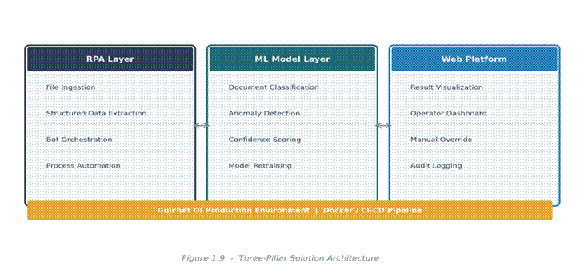
\includegraphics[width=0.85\textwidth,max width=\textwidth]{images/image5.png}
  \caption{Conceptual overview of the FiberGate Ecosystem and its three interdependent components}
  \label{fig:image5}
\end{figure}

\begin{table}[H]
  \centering
  \caption{FiberGate Ecosystem components and the operational problems each addresses}
  \renewcommand{\arraystretch}{1.3}
  \begin{tabularx}{\textwidth}{|X|X|}
    \hline
    \textbf{Component} & \textbf{Operational Problems Addressed} \\ \hline
    SENTINEL Fleet & Repetitive email-driven data entry; copy-paste transcription errors; missed task creation; inequitable distribution; human operational dependency \\ \hline
    FiberGate AI Service & Manual completeness verification; absence of automated CMS file generation; human dependency in document processing \\ \hline
    Unified Platform & Absence of centralized supervision; absence of operational traceability and performance reporting \\ \hline
  \end{tabularx}
\end{table}

The three components are designed to function as a coherent ecosystem. The SENTINEL agents automate the repetitive back-office operations, the AI service provides analytical intelligence over document content, and the web platform serves as the user-facing layer for supervision and decision support. The solution is designed around four architectural principles: reliability, traceability, security, and extensibility. The detailed architecture, technical design, and implementation of each component are developed in the subsequent chapters of this report.

\subsection{Project Objectives and Prioritization (MoSCoW Framework)}

The project objectives were formalized and prioritized using the MoSCoW framework, which classifies each requirement into one of three categories: Must Have, designating requirements critical to project success; Should Have, designating objectives that are important but non-blocking; and Could Have, designating desirable capabilities reserved for future development iterations. This prioritization framework ensures that development resources are concentrated on the most operationally critical capabilities within the constrained twenty-five-week delivery window.

\begin{table}[H]
  \centering
  \caption{Project objectives classified using the MoSCoW prioritization framework}
  \renewcommand{\arraystretch}{1.3}
  \begin{tabularx}{\textwidth}{|X|X|X|}
    \hline
    \textbf{Objective} & \textbf{Description} & \textbf{Priority} \\ \hline
    Full automation of email-driven processing & Eliminate manual handling of POI, CAFF, and distribution emails through automated end-to-end pipelines. & Must Have \\ \hline
    AI-powered document data extraction & Replace manual folder verification with automated field-level extraction and structured recommendation output. & Must Have \\ \hline
    Automated CMS file generation & Generate CMS Excel files automatically from AI-extracted client data without consultant intervention. & Must Have \\ \hline
    Role-differentiated web dashboard & Provide tailored interfaces for Consultant, Pilot, and SDM roles with enforced access controls. & Must Have \\ \hline
    Equitable task assignment & Ensure balanced workload distribution across the 15 OSA consultants through a persistent round-robin routing algorithm. & Must Have \\ \hline
    Reliability and fault tolerance & Guarantee continuous automated operation through retry mechanisms, graceful error handling, and failure alerting. & Must Have \\ \hline
    Operational traceability & Enable auditing and root cause analysis through structured logging of all automated operations. & Must Have \\ \hline
    Security and data protection & Protect sensitive operational data through externalized credentials and secure configuration management. & Must Have \\ \hline
    Operational statistics and supervision & Provide real-time performance dashboards for management-level monitoring and reporting. & Should Have \\ \hline
    Architectural extensibility & Design the solution to support future technology migration, additional connectors, and workload scaling. & Should Have \\ \hline
  \end{tabularx}
\end{table}

\section{Methodology and Project Governance}

This section presents the project governance structure, the hybrid methodology adopted for solution design and delivery, and the execution model that structured the twenty-five weeks of this internship.

\subsection{Stakeholder Identification and Governance Structure}

Effective stakeholder identification constitutes a foundational step in any structured implementation project. Consistent with the PMBOK Guide (Project Management Institute, 2021), stakeholder management requires early identification of all individuals or groups that may affect or be affected by the project outcome. Four distinct stakeholder categories were identified and formally documented in a governance register at the outset of the project.

\begin{table}[H]
  \centering
  \caption{Stakeholder register with governance roles and engagement model}
  \renewcommand{\arraystretch}{1.3}
  \footnotesize
  \begin{tabularx}{\textwidth}{|X|X|X|X|}
    \hline
    \textbf{Stakeholder Category} & \textbf{Representative(s)} & \textbf{Role in Project} & \textbf{Engagement Mode} \\ \hline
    Internal Operational & Guichet OI Team Leads, Production Managers & Validate deliverables at each phase gate; define operational requirements and acceptance criteria & Phase-gate reviews, weekly checkpoints \\ \hline
    Technical and IT & Amaris IT and Infrastructure Team & Manage server access, containerized environments, and security compliance & Consulted on deployment phases \\ \hline
    Academic & University Supervisors & Oversee the research component; ensure thesis alignment with academic standards & Monthly progress reports, thesis review sessions \\ \hline
    End Users & OSA Operators and Consultants & Primary system users; principal source of usability feedback and functional validation & Sprint reviews, structured usability sessions \\ \hline
  \end{tabularx}
\end{table}

A RACI matrix (Responsible, Accountable, Consulted, Informed) was applied across all project activities to clarify ownership and prevent role ambiguity during cross-functional implementation phases. This governance instrument, widely applied in consulting delivery contexts (Harrin, 2022), ensures transparency in decision-making throughout the project lifecycle.

\subsection{Sure Step Hybrid Project Methodology}

The selection of an appropriate project methodology represented a critical early decision. A pure Scrum framework was evaluated but ultimately not adopted, as the consulting context imposes daily production obligations incompatible with fixed-length sprint commitments and fixed team velocity assumptions. The team required a methodology capable of balancing the consulting production rhythm with structured documentation requirements, phase-gated quality control mechanisms, and iterative feedback loops.

The project therefore adopts the Microsoft Dynamics Sure Step methodology, a structured phase-based implementation framework originally developed for enterprise resource planning and customer relationship management deployments. Sure Step organizes the project lifecycle into six sequential phases: Diagnostic, Analysis, Design, Development, Deployment, and Operation. Each phase defines specific activities, deliverables, responsible roles, and quality checkpoints in the form of formal toll-gate reviews that must be passed before advancement to the subsequent phase.

\begin{figure}[H]
  \centering
  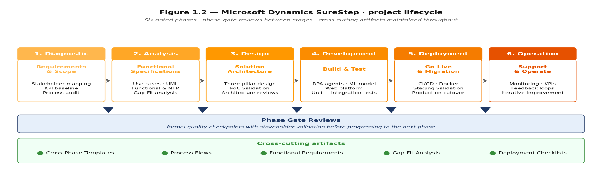
\includegraphics[width=0.85\textwidth,max width=\textwidth]{images/image6.png}
  \caption{The six phases of the Microsoft Dynamics Sure Step implementation framework}
  \label{fig:image6}
\end{figure}

Three characteristics make Sure Step particularly well-suited to this project context. First, its documentation-driven execution model provides templates, process flow diagrams, and deliverable checklists for each phase, ensuring that every design decision is recorded and traceable from requirements gathering through production deployment. Second, its phase-gate quality control mechanism requires formal stakeholder validation of all phase milestones before proceeding, preventing technical debt accumulation and ensuring that validated requirements are not discarded during implementation. Third, Sure Step explicitly supports a hybrid Agile project type, permitting the integration of weekly iteration cycles and incremental deliveries within its phase structure, forming a composite approach compatible with the Guichet OI operational schedule.

\begin{table}[H]
  \centering
  \caption{Comparative evaluation of Sure Step and Scrum across five analytical dimensions}
  \renewcommand{\arraystretch}{1.3}
  \begin{tabularx}{\textwidth}{|X|X|X|}
    \hline
    \textbf{Dimension} & \textbf{Scrum} & \textbf{Microsoft Dynamics Sure Step} \\ \hline
    Planning Horizon & Fixed 2 to 4 week sprints with scope frozen per iteration & Phase-level planning with flexible internal activity scheduling \\ \hline
    Documentation & Minimal by design; the Agile Manifesto prioritizes working software over documentation & Mandatory templates, process flow diagrams, and deliverable checklists per phase \\ \hline
    Role Structure & Three fixed roles: Product Owner, Scrum Master, and Development Team & Flexible phase-level roles: Project Manager, Functional Consultant, and Solution Architect \\ \hline
    Quality Gates & Informal sprint review with Definition of Done applied per user story & Formal stakeholder-validated phase-gate review required before phase transition \\ \hline
    Operational Fit & Optimized for dedicated product teams; poor fit with irregular production workloads & Designed for consulting delivery contexts; absorbs variable production rhythms effectively \\ \hline
    Adoption Decision & Not adopted for this project & Adopted as the base framework \\ \hline
  \end{tabularx}
\end{table}

The most decisive factor in the rejection of pure Scrum was operational compatibility. The Guichet OI production rhythm generates irregular daily workloads correlated with file submission deadlines, rendering sprint velocity unpredictable and sprint commitments unreliable. Sure Step's phase structure absorbs these variations by decoupling phase duration from specific activity sequencing. This analysis is consistent with findings from Conboy and Carroll (2019), who demonstrate that hybrid methodologies consistently outperform pure Agile frameworks in constrained-resource, dual-track operational environments.

\subsection{Project Execution: Phases, Sprint Model, and Timeline}

Each of the six Sure Step phases was mapped to concrete project activities, ensuring a direct correspondence between the methodology structure and execution practice. Within this phase structure, an iterative sprint-based model inspired by Agile practices was embedded. Rather than treating each phase as a monolithic sequential block, phases were subdivided into weekly or bi-weekly cycles, each producing a testable and reviewable increment of the solution.

Each iteration followed a consistent four-step execution pattern. The Observe step involves the identification of a specific production problem encountered during daily processing work. The Formalize step translates the observed problem into structured requirements, use cases, and acceptance criteria. The Implement step involves development of the targeted solution component within the current phase's technical scope. The Validate step consists of testing the component against real production files, followed by stakeholder review and integration into the main solution.

\begin{figure}[H]
  \centering
  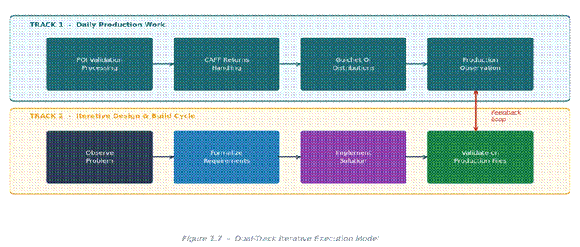
\includegraphics[width=0.85\textwidth,max width=\textwidth]{images/image7.png}
  \caption{Dual-track iterative execution model: Track 1 (daily production) and Track 2 (iterative development)}
  \label{fig:image7}
\end{figure}

\begin{figure}[H]
  \centering
  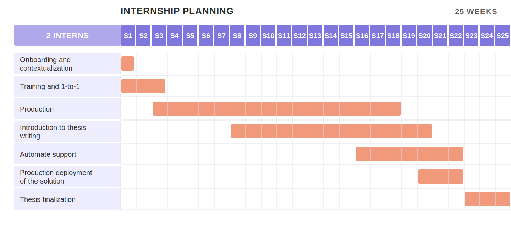
\includegraphics[width=0.85\textwidth,max width=\textwidth]{images/image8.png}
  \caption{Project Gantt chart representing the timeline across the six Sure Step phases}
  \label{fig:image8}
\end{figure}

\begin{table}[H]
  \centering
  \caption{Sure Step phase-to-activity mapping with deliverables and timeline}
  \renewcommand{\arraystretch}{1.3}
  \footnotesize
  \begin{tabularx}{\textwidth}{|X|X|X|X|X|}
    \hline
    \textbf{Phase} & \textbf{Focus Area} & \textbf{Key Activities} & \textbf{Deliverables} & \textbf{Duration} \\ \hline
    1. Diagnostic & Requirements and Scope & Stakeholder mapping, KPI baseline establishment, process audit & Scope document, KPI baseline report & Weeks 1 to 3 \\ \hline
    2. Analysis & Functional Specifications & Use case modeling, UML diagrams, functional and non-functional requirements, Gap-Fit analysis & Functional specification, Gap-Fit report & Weeks 3 to 6 \\ \hline
    3. Design & Solution Architecture & Three-pillar design, proof-of-concept validation, architecture reviews & Architecture document, PoC validation report & Weeks 6 to 9 \\ \hline
    4. Development & Build and Test & RPA agent construction, AI model training, web platform development, unit and integration testing & Working solution components, test reports & Weeks 9 to 17 \\ \hline
    5. Deployment & Go-Live and Migration & CI/CD pipeline configuration, staging validation, production cutover & Deployed system, deployment runbook & Weeks 17 to 21 \\ \hline
    6. Operation & Support and Continuous Improvement & KPI monitoring, operator feedback loops, iterative refinement & KPI dashboard, improvement backlog & Weeks 21 to 25 \\ \hline
  \end{tabularx}
\end{table}

\begin{table}[H]
  \centering
  \caption{Sprint planning summary aligned with Sure Step phases}
  \renewcommand{\arraystretch}{1.3}
  \footnotesize
  \begin{tabularx}{\textwidth}{|>{\raggedright\arraybackslash}p{2.3cm}|X|X|X|}
    \hline
    \textbf{Week Range} & \textbf{Sure Step Phase} & \textbf{Sprint Focus} & \textbf{Expected Output} \\ \hline
    Weeks 1 to 3 & Diagnostic & Onboarding and operational process audit & KPI baseline, stakeholder register, process audit report \\ \hline
    Weeks 3 to 6 & Analysis & Requirements elicitation and system modeling & Functional specifications, use cases, Gap-Fit analysis \\ \hline
    Weeks 6 to 9 & Design & Architecture definition and proof-of-concept & Architecture document, PoC validation report \\ \hline
    Weeks 9 to 13 & Development & Core automation component build & SENTINEL agents version 1, AI model version 1, unit test suite \\ \hline
    Weeks 13 to 17 & Development & System integration and web platform & Integrated system, Unified Platform, integration test suite \\ \hline
    Weeks 17 to 21 & Deployment & Staging validation and production cutover & Deployed production system, deployment runbook \\ \hline
    Weeks 21 to 25 & Operation & Monitoring, feedback integration, and thesis finalization & KPI monitoring report, improvement backlog, final thesis \\ \hline
  \end{tabularx}
\end{table}

\section*{Conclusion}
\addcontentsline{toc}{section}{Conclusion}

This chapter has established the organizational, operational, and methodological foundations upon which the FiberGate project rests. The Amaris--Orange collaboration framework, the specificities of the Guichet OI PAR France unit, and the daily operational realities of the 15-person OSA sub-team collectively define a context characterized by significant and growing processing pressure.

The problem statement analysis has systematically identified nine structural inefficiencies spanning all four manual workflows, each of which is mapped to one or more components of the proposed FiberGate Ecosystem. The solution, structured around the SENTINEL Fleet, the FiberGate AI Service, and the Unified Platform, directly addresses each identified problem through targeted automation, machine intelligence, and centralized supervision.

The governance and methodology section has formalized the project's organizational structure, justified the adoption of the Sure Step hybrid framework over a pure Scrum approach, and established the sprint-based iterative execution model that governed the twenty-five weeks of this internship. The choice of a phase-gated methodology with embedded iterative cycles reflects a deliberate adaptation to the dual constraints of consulting production rhythm and academic rigor.

The subsequent chapter presents the existing system analysis and state of the art, examining the technical foundations of FTTX and PAR engineering, the detailed operational workflows of the Guichet OI unit, and the academic and industrial literature underpinning the three technical pillars of the FiberGate Ecosystem.
